
\documentclass[11pt,a4paper]{article}
\usepackage[utf8]{inputenc}
\usepackage[T1]{fontenc}
\usepackage[spanish,es-nodecimaldot]{babel}
\usepackage[a4paper,left=1.7cm,right=1.7cm,top=20mm,bottom=20mm]{geometry}
\usepackage{amsmath,amssymb,amsfonts,mathtools,bm}
\usepackage{braket}
\usepackage{graphicx}
\usepackage{float}
\usepackage{booktabs}
\usepackage{enumitem}
\usepackage{xcolor}
\usepackage{lmodern,microtype}
\usepackage{fancyhdr}
\usepackage{titlesec}
\usepackage[colorlinks=true,linkcolor=black,urlcolor=black,citecolor=black]{hyperref}
\numberwithin{equation}{section}
\renewcommand{\boxed}[1]{#1}
\setlength{\parindent}{0pt}
\setlength{\parskip}{5pt}
\newcommand{\dd}{\,\mathrm d}
\newcommand{\ii}{\mathrm i}
\newcommand{\e}{\mathrm e}
\newcommand{\hb}{\hbar}
\newcommand{\R}{\mathbb R}
\newcommand{\C}{\mathbb C}
\newcommand{\id}{\mathbb I}

\pagestyle{fancy}
\setlength{\headheight}{14pt}
\fancyhf{}
\fancyhead[L]{\textit{Tarea 16}}
\fancyhead[R]{Mecánica Cuántica I}
\begin{document}
\begin{titlepage}
\centering
\vspace*{1.8cm}

\includegraphics[width=.22\textwidth]{UdeC_escudo.png}
\vspace{1.1cm}
{\Huge\bfseries Tarea 16\par}
\vspace{.4cm}
{\Huge\bfseries Mecánica Cuántica I\par}
\vspace{1.5cm}
{\Large José Ignacio Rosas Sepúlveda\par}
\vspace{.8cm}
{\Large Solución\par}
\vfill
\thispagestyle{empty}
\end{titlepage}
\tableofcontents
\newpage
\section*{Enunciado}
\addcontentsline{toc}{section}{Enunciado}
\begin{enumerate}[label=\arabic*.]
\item Demuestre que los estados propios $\{\ket{\varepsilon_n}\}$ del Hamiltoniano del oscilador cargado, dados en la clase 16, son ortonormales:
\begin{equation}\braket{\varepsilon_n|\varepsilon_{n'}}=\delta_{nn'}.\end{equation}
Use que el operador de desplazamiento $D$ es unitario y que los estados número son ortonormales.
\item Demuestre que
\begin{equation}
\ket{\varepsilon_n}=\frac{1}{\sqrt{n!}}(a^\dagger-\alpha I)^n\ket\alpha,
\end{equation}
donde $\ket\alpha=\ket{\varepsilon_0}$ es un estado coherente.
\item Un oscilador armónico cargado está inicialmente en un estado número $\ket n$.
\begin{enumerate}[label=\alph*)]
\item Encuentre $\ket{\psi(t)}$ expresándolo en la base de estados propios desplazados.
\item Si se mide la energía, indique los resultados posibles y sus probabilidades.
\item Grafique $|\braket{\varepsilon_{n'}|0}|^2$ para $n=0$, $\alpha=1$.
\item Grafique $|\braket{\varepsilon_{n'}|3}|^2$ para $n=3$, $\alpha=6$.
\end{enumerate}
\end{enumerate}


\section{Problema 1}
Los estados propios del oscilador cargado son
\begin{equation}
\ket{\varepsilon_n}=D(\alpha)\ket n,
\end{equation}
con $D^\dagger D=\id$. Entonces
\begin{equation}
\boxed{\braket{\varepsilon_n|\varepsilon_{n'}}
=\braket{n|D^\dagger D|n'}=\braket{n|n'}=\delta_{nn'}.}
\end{equation}

\section{Problema 2}
Para $\alpha$ real,
\begin{equation}
D(\alpha)=\e^{\alpha(a^\dagger-a)},\qquad
\ket\alpha=D(\alpha)\ket0.
\end{equation}
La identidad de desplazamiento
\begin{equation}
D(\alpha)a^\dagger D^\dagger(\alpha)=a^\dagger-\alpha\id
\end{equation}
permite escribir
\begin{align}
\ket{\varepsilon_n}
&=D(\alpha)\frac{(a^\dagger)^n}{\sqrt{n!}}\ket0\\
&=\frac1{\sqrt{n!}}(a^\dagger-\alpha\id)^nD(\alpha)\ket0.
\end{align}
Por tanto,
\begin{equation}
\boxed{\ket{\varepsilon_n}=\frac1{\sqrt{n!}}(a^\dagger-\alpha\id)^n\ket\alpha.}
\end{equation}

\section{Problema 3}
El Hamiltoniano exacto del oscilador cargado posee
\begin{equation}
E_{n'}=\hb\omega\left(n'+\frac12\right)-\frac{q^2\mathcal E^2}{2m\omega^2},
\end{equation}
con
\begin{equation}
\alpha=\frac{q\mathcal E}{\sqrt{2m\hb\omega^3}}.
\end{equation}
Insertamos la identidad en la base desplazada:
\begin{equation}
\ket n=\sum_{n'=0}^\infty\ket{\varepsilon_{n'}}\braket{\varepsilon_{n'}|n}.
\end{equation}
Entonces
\begin{equation}
\boxed{\ket{\psi(t)}=\sum_{n'=0}^\infty
\e^{-\ii E_{n'}t/\hb}\ket{\varepsilon_{n'}}\braket{\varepsilon_{n'}|n}.}
\end{equation}
Si se mide la energía, los posibles resultados son $E_{n'}$ y
\begin{equation}
P_{n'}=|\braket{\varepsilon_{n'}|n}|^2.
\end{equation}
Para $\alpha$ real, esta distribución puede escribirse con polinomios de Laguerre asociados:
\begin{equation}
P_{n'}=\e^{-\alpha^2}\times
\begin{cases}
\displaystyle \alpha^{2(n'-n)}\frac{n!}{n'!}
\left[L_n^{(n'-n)}(\alpha^2)\right]^2,&n'\ge n,\\[7pt]
\displaystyle \alpha^{2(n-n')}\frac{n'!}{n!}
\left[L_{n'}^{(n-n')}(\alpha^2)\right]^2,&n'<n.
\end{cases}
\end{equation}
Para $n=0$ se reduce a una Poisson de media $\alpha^2$.
\begin{figure}[H]\centering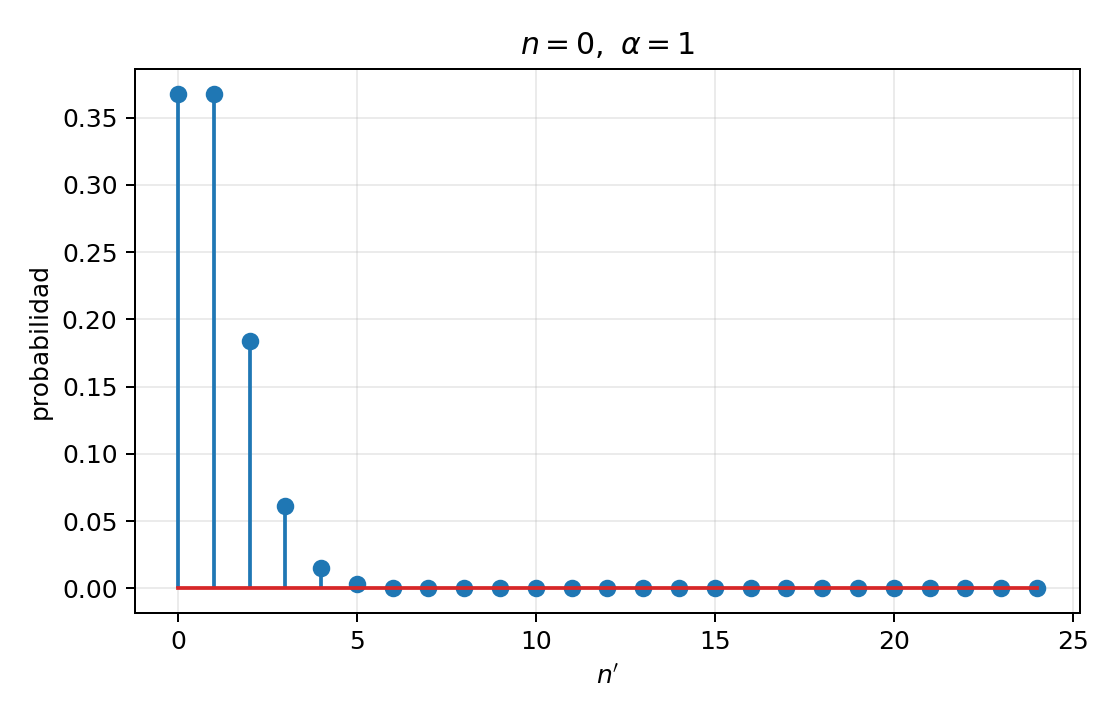
\includegraphics[width=.67\textwidth]{figures/n0_a1.png}\caption{Distribución para $n=0$, $\alpha=1$.}\end{figure}
\begin{figure}[H]\centering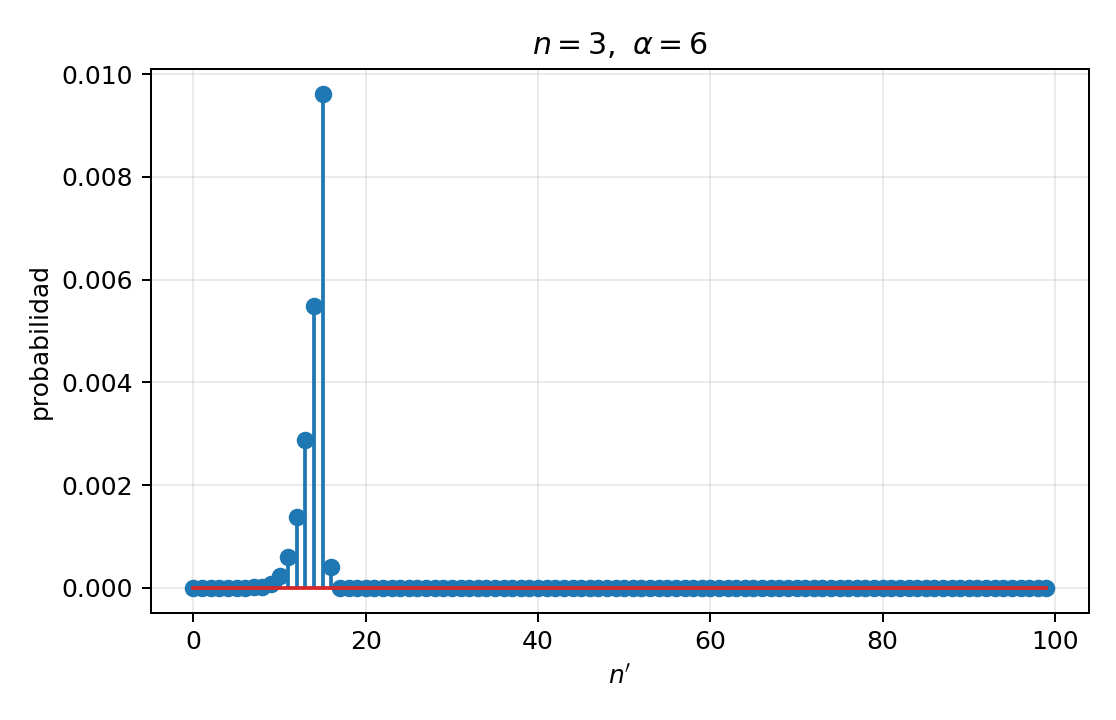
\includegraphics[width=.67\textwidth]{figures/n3_a6.png}\caption{Distribución para $n=3$, $\alpha=6$.}\end{figure}

\paragraph{Comentario.}
Completar el cuadrado en $X$ muestra que el campo desplaza el centro del oscilador y reduce todos los niveles en la misma cantidad $q^2\mathcal E^2/(2m\omega^2)$. La separación entre niveles sigue siendo $\hb\omega$.



\end{document}
